\chapter{Preliminaries}

In this section we present the theoretical background of this work. We first
define the general concept of machine learning, then describe a modern area
of machine learning research --- the automatic machine learning, or AutoML.
Finally, we dedicate two sections to the heuristic optimization method ---
evolutionary computation and its subfield, genetic programming.

\section{Machine learning}
The field of machine learning, shortly ML, encompasses a broad range of
algorithms and statistical methods for data processing. In his book on machine
learning, Flach provides the following general definition:

\blockquote{Machine learning is the systematic study of algorithms and systems
that improve their knowledge or performance with experience
\citep{Flach:2012:MLA:2490546}.}


The knowledge of a system is gained through learning from \emph{experience}.
This procedure is referred to as the \emph{training} phase. In this process, 
the ML system adjusts its parameters according to the nature of training data.
The result of the process is a prediction function which depends on learned
parameters. By applying this function on previously unseen data, denominated 
as the \emph{testing} data, we obtain the output of the algorithm. The 
result is then evaluated to determine the performance of the method 
\citep[p.~2]{Bishop:2006:PRM:1162264}. The character of the learning process
varies with different machine learning problems. There are three main classes 
of tasks: \emph{supervised}, \emph{unsupervised} and \emph{reinforcement} 
learning.

In case of supervised learning, the training data is a set of labelled examples
(also called instances)
and the task is to predict labels of previously unseen data. The field is 
further subdivided into two groups. If the labels are elements of a finite 
number of discrete categories, the problem is called \emph{classification}. 
The continuous case is then called \emph{regression}.
In contrast to supervised learning, in unsupervised learning the training data 
is unlabelled. The key task is then to divide the data into groups of 
similar examples. The task of reinforcement learning is to find suitable
actions as to maximize a reward. The training data is in this case a history of
previous actions and corresponding rewards \citep[p.~3]{Bishop:2006:PRM:1162264}.

In the following sections we elaborate on some important concepts of machine
learning. We will focus on supervised learning.

\subsection{Performance of machine learning models}
In this section we describe the general terms related to performance evaluation 
of machine learning models. We first present a formal 
definition of supervised learning \citep{Russell:2009:AIM:1671238,
Mitchell:1997:ML:541177}.

\begin{definition}[Supervised learning]
Let $X\subset\tilde{X}$ be a set of examples (or also \emph{feature vector})
from an unknown space and $y\subset\tilde{y}$ a set of corresponding labels.
Moreover, let $f: \tilde{X} \rightarrow \tilde{y}$ be an unknown function that
satisfies $f(X) = y$.
Then the task of \emph{supervised learning} is to find a hypothesis function
$h$ which approximates the function $f$ by \emph{learning} from the training
set $(X,y)$.

\end{definition}

Suppose we have a model which learned a particular hypothesis $h$ and we want
to determine whether it approximates $f$ well. In other words, we want to
measure the difference between the output of the model and the real value of
the target --- the \emph{error} of the model. There are several types of
metrics that can be used as error functions. In case of classification, the
simplest metric is the \emph{error rate} which is defined as the proportion of
incorrectly classified instances --- examples $x$ for which $h(x)\neq y$.
A related term is the \emph{predictive accuracy}, which is defined as the
proportion of correctly classified examples
\citep[p.~54]{Flach:2012:MLA:2490546}.

The performance of a model is thus tied with a small error rate. However, it is
important to note that good performance on training data does not ensure 
just as good performance on new data. Sometimes the model performs 
exceptionally well on training data, but fares much worse on testing data. 
This behaviour is called \emph{overfitting} and usually occurs when 
unnecessarily subtle details of the data are learned. The opposite concept 
is called \emph{generalisation}, which is the ability to perform well on 
different types of testing data.

A related term is so-called \emph{bias-variance dilemma}, which is a phenomenon
closely related to model selection. The bias and variance of a model are
defined as follows \citep[p.59,~356]{CaseBerg:01}

\begin{definition}[Bias and variance]
Bias of a model is the value $E(h_t(X)) - y$, where $h_t$ is a
hypothesis learned from a particular training set $t$ and $X$ and $y$ is the
set used for evaluation. Variance of a model is defined as $E[(h_t(X) - y)^2]$.
\end{definition}

Practically, a model with few parameters will make some errors even with
sufficient training data, thus introducing a bias from the correct output.
On the other hand, by  increasing the number of model parameters, it will
highly depend on training data. Then, with small changes in data there will be
a high variance in the output. A model with both small bias and small variance
can rarely be found, hence it is often necessary to choose the side that is
less harmful to the particular task. Another option
is to use some of the ensemble methods described in section \ref{ensemble}. For
example, \hyperref[bagging]{bagging} is a method of variance reduction, while
\hyperref[boosting]{boosting} noticeably reduces the bias
\citep[p.~93--94,~338]{Flach:2012:MLA:2490546}.

The task of finding a model which performs well on a particular problem
instance is by no means straightforward. In practice, it is usually solved by
iterative selection of model settings. As described in section \ref{sec:automl},
there are systems which automatize a part of the process. Nevertheless, even
these methods must take into account the problems presented in this section.

\subsection{Model ensembles} \label{ensemble}
Model ensembles are powerful learning techniques that combine simpler models 
to achieve better results. They are widely used in practice, specific examples
can be found in the review of \cite{Rokach:2009:TCE:1609202.1609436}.

The rationale behind ensembles is also of theoretical character, namely from
statistics and from computational learning theory. In statistics, a general
idea is to average measurements to get more stable and reliable results.
Here, the models are trained on data samples or feature subsets and the results
are then combined into a final hypothesis.
% Flach TODO cite

The computational learning theory defines the term \emph{learnability},
which describes whether a model outputs a correct hypothesis by learning on
random sets of instances from a unknown distribution. A \emph{strong learner}
is a model which outputs most of the time a correct hypothesis. It is not
required that it always produces a hypothesis with error equal to zero, as 
the set of chosen instances might be atypical or not representative enough.
Similarly, a \emph{weak learner} is then a model which outputs most of the time
a hypothesis, which is slightly better than random guessing (i.e. has a
success rate over 0.5). A more detailed elaboration of the learnability
theory is beyond the scope of this work and can be found in books 
of \citep{Flach:2012:MLA:2490546} and \citep{Mitchell:1997:ML:541177}.

The assumption of strong learnability may appear to be quite strict when 
compared to the weak learnability, as the model must output a correct 
hypothesis on almost all example sets. However,
\cite{Schapire:1990:SWL:83637.83645} proved that a model 
is weakly learnable if and only if it is strongly learnable. 
 This was proven in a constructive manner
by iteratively correcting the errors of the hypotheses, thus \emph{boosting} 
the model. The boosting method has directly inspired one of the most successful
ensemble methods --- the award winning AdaBoost.
\citep{Freund:1996:ENB:3091696.3091715, Freund:1997:DGO:261540.261549}

In the following sections, we will present some of the most used ensemble 
methods.
\phantomsection
\paragraph{Bagging} \label{bagging}
\emph{Bootstrap aggregating}, usually abbreviated to bagging, is a highly
effective ensemble method. First, $n$ samples are independently taken from 
the original dataset with replacement. This is referred to as 
\emph{bootstrapping}. Then, we use the samples to train an ensemble of $n$
different models. It can be used to generate predictions, which are
then \emph{aggregated} by voting or averaging into a final prediction.

This method takes advantage of the statistical stability described at the
beginning of this section. As the examples are drawn with replacement, there
will be some instances missing in every sample. Thus, we introduce diversity
between the ensemble models. \citep[331]{Flach:2012:MLA:2490546}

\phantomsection
\paragraph{Boosting} \label{boosting}
The above-mentioned boosting technique uses a different approach to model
combining. Before the learning process starts, we add weights to the training 
examples (the base-learner must support weighting). Then, we learn the model
on the modified training set, which produces a set of misclassified instances
along with the (weighted) training error. We then adjust the weights in such a
way that weights of the correctly classified examples decrease and those of
the incorrectly classified examples increase. Therefore, when we continue and
learn a new model on the data with changed weights, it will concentrate more 
on the problematic instances.

The algorithm stops after a fixed number of iterations or when the weighted
training error increases over $0.5$ --- which is when the algorithm stops
improving. The resulting prediction is again an average of all model
predictions, but with putting more weight on models with a lower training
error. \citep[335]{Flach:2012:MLA:2490546}

\section{AutoML} \label{sec:automl}
When using machine learning in practice, it is not always evident which model
is suitable for a particular problem. As a consequence of the `no free lunch'
theorem \citep{585893}, it is not possible for a single ML algorithm to
outperform all other methods for an arbitrary problem instance. As such, model
selection and hyperparameter choice must be performed in order to obtain a 
satisfactory result. Along with this, it is necessary to use more complex
models for some ML problems. For example, we may use some of the ensemble
methods which reduce bias or variance (section \ref{ensemble}). Also, the data
typically requires some preprocessing before it can be passed to a ML
algorithm, hence the model becomes even more complex. All these aforementioned
tasks require human  expertise and are usually time-consuming. The automated
machine learning --- AutoML --- aims to automatize the process and make
machine learning available even to non-experts \citep{Zller2019SurveyOA}.
% TODO internet source - AutoML page

There seems to be no generally accepted definition of AutoML as for now.
According to \cite{DBLP:journals/corr/abs-1810-13306},
\textquote{\textit{AutoML attempts to construct machine learning programs
\ldots without human assistance and within limited computational budgets.}}
Informally, AutoML encompasses methods that automatize a part of a machine
learning workflow. Examples of existing AutoML systems are presented in chapter
\ref{ch2:related}.

\subsection{Machine learning workflows}
A machine learning workflow is the process of solving a particular machine
learning problem. In literature, it is also labelled as a `machine learning
pipeline' \cite{DBLP:journals/corr/abs-1810-13306}. However, in the context
of AutoML it may not be a suitable term, as a pipeline is a set of methods
logically arranged into a directed acyclic graph (DAG), but the workflow itself
is an iterative process, as can be seen in Figure \ref{pic01:workflow}.
The term \emph{pipeline} generally denotes complex model structures which
comprise several feature preprocessing methods and/or model
ensembles.

A workflow can be decomposed into well-defined steps, which are depicted in
Figure \ref{pic01:workflow}. The formulation of the problem and data collection
is usually performed by an expert from an unrelated field, whereas the rest is
the task of a machine learning scientist. The feature engineering comprises
of initial data cleaning and feature extraction.
After that, a suitable machine learning model must be selected along with
suitable hyperparameters. Finally, the resulting model is evaluated, most
often on a set of previously unseen \emph{validation data}.

\begin{figure}[ht]\centering
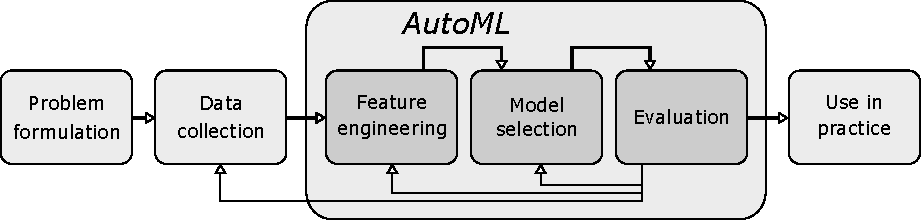
\includegraphics[width=\textwidth]{../img/workflow-pdfa.pdf}
\caption{A typical machine learning workflow}
\label{pic01:workflow}
\end{figure}

The process of solving the problem is iterative; it is usually necessary to try
out many different settings, as there are no algorithms that would perform
well on all types of problems.
There are many possibilities in what to optimize. Some models concentrate only
on one part of the workflow, for example on automatic feature engineering,
other handle multiple steps at once. As mentioned above, there is no general
categorization % hierarchy? better word?
of AutoML frameworks. Thus, in the following sections we present only some
AutoML approaches relevant to this work. For more examples and a proposition
of a general AutoML framework refer to \cite{DBLP:journals/corr/abs-1810-13306}.

\subsection{Hyperparameter optimization}
Automated hyperparameter optimization (HPO) is the most basic, but nevertheless
very important task of AutoML. In the simple case, HPO is the task of finding
a hyperparameter setting of a machine learning algorithm that performs
the best on a given dataset. If we optimize multiple models at once, we obtain
an extended version of this problem --- combined algorithm selection and
hyperparameter optimization problem, or CASH for short. The task is then to
select the best combination of model and hyperparameter setting
\citep{DBLP:journals/corr/abs-1208-3719}.

By combining multiple hyperparameter spaces, we optain a very large search
space of possible models. There are several limitations which complicate the
search through this space. For large models (for example in deep learning)
and large datasets, the learning process and evaluation take a lot of time.
Moreover, the configuration space may be quite complex, with many continuous
hyperparameters or some which depend on each other. It is also necessary to
avoid overfitting, which is not always obvious as the training set may not be
large enough.

Some examples of frameworks which try to solve the HPO are mentioned in section
\ref{ch2:related}. Various approaches are presented in the book written by
\cite{automl_book}.

\subsection{Creating model architecture} \label{sec:modelarch}
The creation of model architecture is a problem related to the HPO. It is an
important part of the design of neural networks, which is currently a very
popular area of research --- neural architecture search (NAS). It also needs
to be considered in traditional machine learning when employing model ensembles
or several feature preprocessing methos.
The problem may be solved at the same time as HPO, which however introduces
even more complexity in the search space.

There are many difficulties that have to be solved when designing automated
architecture search methods. With increasing size of the search space 
the optimization time may become very long.
Moreover, some complex models may score only slightly better
but at the cost of a considerably longer running time. Also, evaluation cost of
a single model may be very high, preventing the AutoML system from being usable
in practice.

The \hyperref[metalearning]{metalearning}, which uses \emph{metaknowledge}
about previous results of machine learning algorithms (as described in the
following section), can be very useful in the process. It enables us to
select models which performed well on similar datasets, thus starting with
promising models instead of spending time on poor ones. This approach
significantly speeds up the optimization process and possibly improves the
result \citep{DBLP:journals/corr/abs-1810-03548}.
Another option is to estimate the performance of the architecture. There are
various approaches. For example, we can evaluate the model on smaller subsets of
data, which however introduces some bias in the estimate. Another option is to
decrease the training time, if it is possible, and extrapolate the learning
curve. More on this topic is described in a recent survey by
\cite{2018arXiv180805377E}.

\subsection{Metalearning} \label{metalearning}
The metalearning, also known as `learning to learn' is a field closely related
to AutoML. The subjects of study of this approach are universal properties of 
data and the learning process itself. Just as in case of the traditional
learning --- or also \emph{base-learning} --- metalearning improves with
experience. The difference lies in the learning process. While base-learning
comprises of a single run on a specific task, metalearning may include a
several runs or many different tasks. 

One of the applications of metalearning is model recommendation. The input
data is most frequently a history of previous runs. First, we need to
accumulate some \emph{metadata} to learn from. Mostly, the metadata contains
algorithm performance from past runs and \emph{metafeatures}, which are
artificial features based on characteristics of input datasets. Using the
\emph{metaknowledge} learned from the metadata, we can choose an algorithm that
performed well on datasets whose metafeatures are similar to those of our
dataset.

There are many other concepts used in metalearning; some are presented in more
detail in following chapters, others can be found in the book by
\cite{Brazdil:2008:MAD:1507541} or in a recent survey by
\cite{DBLP:journals/corr/abs-1810-03548}.

\section{Evolutionary computing} \label{ea}
Evolutionary computing is a heuristic optimization method inspired by 
Charles Darwin's theory of \emph{natural selection}. \cite{darwin} In 
a population, individuals with the best characteristics are most likely
to reproduce, thus passing the traits to the offspring. As the 
evolution is repeated over several generations, the most advantageous traits 
predominate. This phenomenon is also called `survival of the fittest'.

In an evolutionary algorithm, the goal is to find the ``best'' solution 
to the given problem by optimizing a \emph{objective function}. The term
`population' refers to a set of solutions encoded as chromosomes which 
represent the defining features of a particular solution. This corresponds
to the genotype--phenotype relationship from genetics. The `natural selection'
can be then understood as a stochastic search through the space of possible 
chromosome values. 
(\cite{Engelbrecht:2007:CII:1557464})

% Maybe a better section name
\subsection{Evolutionary algorithms in detail}
As can be seen in algorithm \ref{alg:EA}, a genetic algorithm should 
define a suitable \emph{selection} method, \emph{mutation} and/or 
\emph{crossover} operators and a \emph{fitness function}.
The algorithm terminates when some \emph{stopping condition} is met. 

\paragraph{Selection}
The selection may be divided into two steps. The first is the 
\emph{parent selection}, also called \emph{mating selection}
(line \ref{parent:sel}), and the second is called
\emph{environmental selection} or \emph{recombination} (line \ref{envir:sel}).
Sometimes the latter is omitted, as the selection can be limited to copying 
all offspring to the new population.

The purpose of the parent selection is to select individuals for the
mating process. Usually, it is a probabilistic process with `better'
individuals being more likely to be selected. The worse individuals have some
chance to be selected as well for the sake of maintaining diversity in the
population. An example of the mating selection is the
\emph{tournament selection}, where individuals `compete' in rounds and the
overall winner is selected. A round is won by an individual, if it has a 
greater fitness value.

The environmental selection is used to create a new 
population. Unlike the mating selection which is a stochastic process,
replacement is usually deterministic. Individuals with a higher fitness are
usually preferred as in the first type of selection, but the decision may take 
into account the age of the individuals. As such, it is possible to include 
or not to include the parents along with the offspring. A popular option is to 
directly choose a small number of the most successful individuals. This method 
is called \emph{elitism} \citep{Eiben:2015:IEC:2810085}.
An example of an elitist selection algorithm is NSGA-II, which
is described in section \ref{nsgaii}.
% TODO cite pages directly, when citing from a single source for several
% paragraphs?

\paragraph{Crossover and mutation}
The crossover and mutation (also called reproduction operators
\citep{Engelbrecht:2007:CII:1557464}) are genetic operators that modify the
structure of individuals to create new ones. Both operations are highly
dependent on problem encoding, as they directly alter the genomes. An example
of the operators can be found in section \ref{gp:treebased}. In the schema 
of the \hyperref[alg:EA]{evolutionary algorithm} (EA), reproduction operators
are applied on parents selected by the mating selection, as can be seen on 
lines \ref{crossover} and \ref{mutation}.

During the crossover, the genetic information of the parents is combined into
one or more children. Most usually, two parents are used to produce two
offspring, though the counts may differ in some special types of evolutionary
algorithms. Ideally, if we have two parents with different but nevertheless
`good' features, the offspring receives both of them.
\citep{Eiben:2015:IEC:2810085}

The mutation is a stochastic operator which is used to introduce diversity into
the population. The structure of the genome is randomly changed in the hope
of creating a more fit individual. Thus, it must be applied with care, as it is
also possible that some good part may be distorted in the process. This can be
avoided by setting a low mutation probability or by elitism.

\paragraph{Stopping criteria}
Some commonly used stopping criteria, as listed by Engelbrecht, are for example 
a limit on the number of generations, a objective function threshold or
termination after no improvement is observed.
(\citep{Engelbrecht:2007:CII:1557464})


\begin{algorithm}
\DontPrintSemicolon 
\caption{Evolutionary algorithm\label{alg:EA}}
  \KwData{population size $k$, stopping condition $c$, 
          crossover probability $p_{cx}$ and mutation probability $p_{mut}$}
  \KwResult{evolved individuals}
  \SetNoFillComment
  \SetKwFunction{Cx}{crossover}
  \SetKwFunction{Mut}{mutation}
  \;
  $P(0) \longleftarrow$ population of size $k$

  \While{$c$ is not met}{
      \For{individual $ind$} {
         $f(ind) \longleftarrow$ compute fitness
      }
      \;
      \tcc{reproduction}
      \For{i in \Range{$k/2$}} {
         $i_1, i_2 \longleftarrow$ select two individuals from $P(n)$\label{parent:sel}

         \If{$p_{cx}$} {
            \Cx{$i_1, i_2$} \label{crossover}
         }
         
         \If{$p_{mut}$ for $k=1,2$} {
            \Mut{$i_k$} \label{mutation}
         }
         \;
         add $i_1, i_2$ to offspring population $P_o(n)$
      }
      \;
      $P(n+1) \longleftarrow$ select $k$ individuals from $P_o(n)$ \label{envir:sel}
  }
  \;
  \KwRet{$P(c)$}  
\end{algorithm}

The advantage of genetic algorithms is such that there are potentially 
many different solutions present in every population. With well defined 
selection and fitness, the algorithm performs a multi-directional search. 
In comparison with other directed search methods, this proves to be a more 
robust approach. (\cite{Michalewicz:1996:GAD:229930}, 
\cite{Mitchell:1997:ML:541177}) % Mitchell page 260 TODO

\subsection{Multi-objective optimization} \label{moo}
In many problems, the quality of the solution depends on more than one
objective function. With this, it is much harder to say whether one solution
is strictly better than another. Multi-objective optimization (MOO) formally
describes this class of problems. We first define the general terminology
and then present MOO in evolutionary computation.

In an optimization problem, the task is to maximize or minimize the objective
function $f(x)$, where $x$ is a vector from the search space. The problem may
also be restricted by constraints in the form of equalities and inequalities.
In multi-objective optimization, the setting remains the same, but the
objective function changes to an \emph{objective vector} ---
for objective functions $f_i(x), i = 1,\ldots,k$, the objective vector is 
defined as $f(x)~=~(f_1(x), f_2(x), \ldots, f_k(x))$.

Although the problem setting is similar, the meaning of optimality needs to 
be redefined. For once, given a pair of solutions, one solution may be better 
than the other solution in one objective function and worse in another. For 
this purpose, we need the following definition.

\begin{definition}[Domination]
In a minimization problem, a vector $x_1$ dominates a vector $x_2$ if and 
only if 
\begin{compactitem}
\item $\forall i=1,\ldots,k: f_i(x_1) \leq f_i(x_2)$, and
\item $\exists j=1,\ldots,k: f_j(x_1) < f_j(x_2)$
\end{compactitem}
\end{definition}

As it is possible to have solutions where neither one dominates the other,
it is impossible to determine one optimal solution. Hence we define the 
\emph{Pareto-optimality}
\citep[p.~551-561,~569--573]{Engelbrecht:2007:CII:1557464}.

\begin{definition}[Pareto-optimality]
A vector $x_1$ is said to be \emph{Pareto-optimal}, if there is no other vector
$x_2$ that dominates it. The \emph{Pareto-optimal set} $P^*$ is the set of all
non-dominated solutions. Finally, the \emph{Pareto-optimal front} (Pareto front)
is defined as
$PF^* =\{\, f=(f_1(x^*),\ldots f_k(x^*)) \mid x^* \in P^* ) \,\}$. 
\end{definition}

If we use evolutionary computation to solve multi-objective problems, the
algorithm needs to be modified. As not every individuals are directly
comparable, we cannot use the selection operators defined in
\ref{ea}. As such, there are various approaches on how to solve this problem,
which can be divided into three groups:

\begin{compactitem}
\item Weighted aggregation --- define a single objective function as a weighted
sum of sub-objectives and proceed with standard evolutionary algorithm
\item Population-based non-Pareto solutions --- works with the sub-objectives,
but does not use the dominance
\item Pareto-based solutions --- tries to approximate the Pareto front
\end{compactitem}

From these three groups, we describe in more detail one Pareto-based algorithm.
More examples are presented in 
\cite[p.~170-173]{Engelbrecht:2007:CII:1557464}.
The algorithm is called Nondominated sorting genetic algorithm (NSGA). It is a
\emph{ranking} selection, which means that individuals are sorted by their
fitness values and the selection is performed with regard to the ordering.

To compute the fitness, the individuals are divided into non-dominated fronts.
This is done by finding a Pareto front of a subpopulation, assigning a
front number to its individuals and removing the from the subpopulation.
The process is repeated with front numbers increasing until no unassigned
individuals remain. Every front then obtains a dummy fitness value, where
the fitness of a front $F(n)$ is better than the fitness of $F(n+1)$. Moreover,
for every individual the value is divided by a \emph{niching} factor (while
keeping the fitness inequality). The 
niching factor is defined as
$$N(i)=\sum_{j\neq i}{S(d((i,j))}$$ where 
\begin{equation}
    S(d(i,j))=
    \begin{cases}
      1 - (\dfrac{d(i,j)}{\sigma_{share}})^2, & \text{if}\ d(i,j) < \sigma_{share} \\
      0, & \text{otherwise.}
    \end{cases}
\end{equation}
This is the definition from the original article of
\cite{Srinivas:1994:MOU:1326668.1326671}, but it can be computed in a different
manner, for example as the count of individuals closer than $\sigma_{share}$
\citep{Engelbrecht:2007:CII:1557464}.

\label{nsgaii}
As the algorithm has some drawbacks, like dependence on $\sigma_{share}$,
a very high computational complexity and lack of elitism, the authors of
NSGA have proposed an improved variant called NSGA-II. This algorithm not only
adresses the above-mentioned problems, it also outperforms other elitist
algorithms \citep{Deb:2002:FEM:2221359.2221582}.

\section{Genetic programming}
% TODO GP and dev-GP applications
In this section, we present a subfield of evolutionary computing --- 
the genetic programming (GP) --- where the population is a set of computer 
programs. The aim of this technique is to evolve programs that provide 
a good solution to the given problem. There are various approaches in means 
of how to represent the individuals and what kind of genetic operators to 
use.

\subsection{Tree-based genetic programming} \label{gp:treebased}
The individuals are most frequently represented in the form of 
\emph{syntax trees}. Inner nodes of the tree are \emph{functions}, whereas 
leaves  are constants (\emph{terminals}) and variables. Together, all possible
functions and terminals form the \emph{primitive set}. Every function of the
set must have a well-defined arity value.

An extension of the genetic programming is \emph{strongly typed GP}. It
constraints the primitive set in such a way that every primitive has an output
type and furthermore every function defines input types of its arguments.

The initialization step is very important, as
there are many different ways how to design trees. Also, specialized genetic
operators need to be designed. On the other hand, the selection step remains
largely the same. \cite{Poli:2008:FGG:1796422}
 
The fitness is usually computed by running the program and comparing the result 
with the desired output. It is also possible to apply genetic programming on
multi-objective problems, where the second objective may be the running time
of the problem or some other domain-specific property
\citep{Poli:2008:FGG:1796422}. More about multi-objective optimization can be
read in section \ref{moo}.

\paragraph{Initialization}
During the initialization, the nodes of the tree are selected from the
primitive set which is provided as input to the algorithm
\citep{Koza:1992:GPP:138936}. As was mentioned, there are various methods of 
initialization. We well present two methods that are among the simplest and 
most used ones --- \emph{grow} and \emph{full}.

In both cases, nodes are inserted to the tree up to a certain height limit.
The two methods differ only in the way how nodes are selected. The grow method
allows to select both functions and terminals before the limit is reached;
afterwards, only terminals can be inserted. The full method restricts the
selection only to functions on all levels but the last one, thus generating 
a full tree. Leaves are then
chosen from the terminal set like in the previous approach.

The drawback of the full method is that all trees are very similar. On the
contrary, the grow method generates a wide range of sizes and shapes, but the
number of nodes in a tree might be too small. Because of that, a method called
\emph{ramped half-and-half} is often used in practice. It combines both 
of the presented methods; half of the population is generated using the full
method, the other one via grow method. Also, instead of one height limit, a
range of values is used to introduce more diversity.
\citep{Poli:2008:FGG:1796422}

\paragraph{Genetic operators} \label{treeops}
The most common type of crossover is \emph{subtree crossover} of two
individuals. A random node --- the crossover point ---
is selected in each individual independently. Then, subtrees corresponding
to the points are exchanged between them.

Similarly, the most used mutation technique is \emph{subtree mutation}.
Just like in subtree crossover, a mutation point is randomly chosen.
Afterwards, the corresponding subtree is entirely replaced by a new randomly
generated tree. Another possibility is to swap a node with a different one
from the primitive set. In the case of strongly typed GP, both input an output
types must match the types of the previous node.
\citep{Poli:2008:FGG:1796422}

\subsection{Developmental genetic programming} \label{devGP}
In simple GP, it is not possible to directly evolve other graph structures
than trees. There are other types of GP that enable this, but individuals
and genetic operators may become fairly complex. However, there is also a
subfield of tree-based GP --- developmental GP --- which allows to indirectly
evolve not only arbitrary graphs, but also much more complex real-world
structures.

The key concept of the developmental genetic programming is the
specific \emph{cellular encoding} of individuals. It was first presented by
\cite{Gruau:1994:thesis} as a form of evolution of neural network architecture.
In cellular encoding, an \emph{embryo} is a basic structure from which all
individuals are created.
The root of the GP tree responds to this cell and every subtree corresponds
to operations which modify specific parts of the cell. In the case of neural
networks, these operation are for example node insertion or parallel/serial
duplication of a part of the network. John Koza has used the developmental GP
to evolve analogue circuits \citep{Koza:1998:circuits}. With this, it was even
possible to achieve human-competitive result, that is, reinventing a circuit
that has been previously designed for a specific purpose by hand.

More about the encoding and modifying operations will be presented in
chapter \ref{our:solution}.